Il modello M/M/1 \`e un caso particolare di M/G/1, in cui gli arrivi e il servizio sono markoviani (o senza memoria). I tempi inter-arrivo sono variabili aleatorie esponenziali con tasso $\lambda$. Stessa cosa dicasi per il servizio, con la differenza che i tempi hanno tasso $\mu$.
Per i calcoli dei momenti delle metriche, si consiglia di vedere~\cite[546-552]{libro:tele}.\\
Nell'articolo~\cite{art:MM1}, si utilizza un sistema M/M/1 per calcolare il tempo totale di conferma di un blocco, che \`e pari alla somma del tempo di generazione (tempo impiegato dal processo di mining) e il tempo dovuto al consenso e all'aggiunta nel registro. 
Questo articolo, però, \`e poco rigoroso nel presentare le ipotesi e i procedimenti matematici che portano ai risultati finali. Infatti, le ipotesi si basano su quelle dell'articolo~\cite{art4:GM1}, in cui si fa riferimento al modello G/$M^B$/1, che ha la particolarità di avere un \textit{batch service}. Questa ipotesi, non viene specificato in~\cite{art:MM1}. Mentre, per quanto riguarda i procedimenti matematici, dall'eq. 6 in~\cite[sez. 3]{art:MM1}, viene utilizzato il parametro $m$, che viene definito come il \textit{numero di servitori nel sistema}. Inoltre, dopo l'eq. 7 in~\cite[sez. 3]{art:MM1}, viene posto $m=2$ senza specificare il motivo di tale scelta.

%**************************************************************
\section{M/M/1 vs m$\times$M/M/1}
Il modello che più si addice alla descrizione del processo di mining \`e m$\times$M/M/1, ovvero un modello in cui ci sono $m$ minatori, i quali hanno ciascuno una coda M/M/1. Se supponiamo che ogni coda abbia un tasso degli arrivi pari a $\lambda$ e un tasso di servizio pari a $\mu$, allora il modello complessivo \`e ancora markoviano e ha tassi rispettivamente pari a $\frac{\lambda}{m}$ e $\frac{\mu}{m}$.
Per osservare le prestazioni dei due modelli, \`e utile confrontare i loro tempi medi totali $m_s$, che sono pari a~\cite[564]{libro:tele}:
\begin{itemize}
\item per M/M/1
\begin{equation}m_{s_1}=\frac{1}{\mu - \lambda}\end{equation}
\item per m$\times$M/M/1
\begin{equation}m_{s_2}=\frac{m}{\mu - \lambda}\end{equation}
\end{itemize}
Nella fig.~\ref{im:confronto} \`e mostrato il grafico che confronta le prestazioni dei due modelli, assumendo $m=20$ e $\mu=1$.
\begin{figure}
\centering 
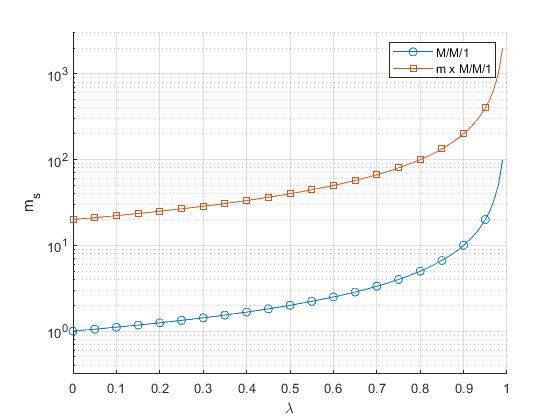
\includegraphics[scale=0.76]{immagini/confronto} 
\caption{Tempo medio di sistema $m_s$ in funzione del tasso degli arrivi $\lambda$ dei due modelli, assumendo $m=20$ e $\mu=1$}
\label{im:confronto} 
\end{figure}
Il grafico mostra l'andamento del tempo medio totale $m_s$ in funzione del tasso degli arrivi $\lambda$. Si può notare che m$\times$M/M/1 \`e la soluzione peggiore in quanto, avendo $m$ minatori che lavorano in parallelo, \`e altamente probabile che qualcuno di loro sia impegnato e qualcun altro non lo sia. Nel caso M/M/1, invece, la coda \`e unica e quindi l'unico minatore che c'\`e, rimane sempre impegnato finch\`e \`e presente qualcuno in coda. Dunque, una transazione (o un blocco) richiede un tempo complessivo maggiore con il modello m$\times$M/M/1 perch\`e, oltre ad aspettare in coda, deve attendere un tempo medio più lungo in servizio perch\`e, per ipotesi, il minatore \`e lento (ha un tasso di servizio pari a $\frac{\mu}{m}$ anzich\`e $\mu$).

%**************************************************************
\section{Analisi del processo delle partenze}
Un altro vantaggio dell'utilizzo del modello M/M/1, risiede in un teorema che si riferisce al processo delle partenze da un sistema M/M/1 stabile. Questo teorema \`e il seguente.
\begin{teorema}[di Burke] 
Il processo delle partenze da un sistema M/M/1 stabile \`e poissoniano di parametro $\lambda$.
\end{teorema}
Il fatto che il tasso di uscita sia $\lambda$ \`e dovuto alla stabilità del sistema. Il teorema di Burke dice una cosa più forte, ovvero che il processo delle uscite \`e poissoniano, quindi senza memoria. Questa proprietà può essere utilizzata per descrivere, sempre con un modello M/M/1, il \textit{consenso}, ovvero quel processo che avviene dopo il mining. Quindi, possiamo rappresentare i due processi di mining e consenso come una \textit{cascata di due code M/M/1 stabili e indipendenti}, in cui valgono tutte le proprietà già note sui singoli sistemi. Questo, \`e sicuramente un beneficio rispetto all'utilizzo di altri modelli, nel caso in cui si voglia analizzare (indipendentemente dal mining) anche il consenso.
